%(BEGIN_QUESTION)
% Copyright 2006, Tony R. Kuphaldt, released under the Creative Commons Attribution License (v 1.0)
% This means you may do almost anything with this work of mine, so long as you give me proper credit

Skriv ligninger som uttrykker totalspenningen indikatoren måler, som funksjon av spenningene vist i diagrammene. Anta at alle skjøter er samme termoelementtype (f.eks. alle type J, alle type K osv.):

$$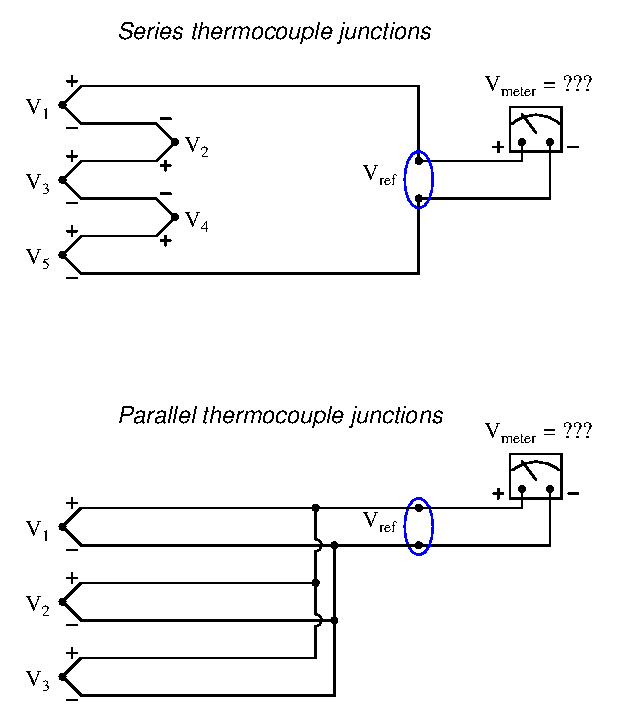
\includegraphics[width=15.5cm]{i00399x01.eps}$$

\underbar{file i00399}
%(END_QUESTION)





%(BEGIN_ANSWER)

\noindent
{\bf Serie:}

$$V_{meter} = (V_1 + V_3 + V_5) - (V_2 + V_4 + V_{ref})$$

\vskip 10pt

\noindent
{\bf Parallell:}

$$V_{meter} = {{V_1 + V_2 + V_3} \over 3} - V_{ref}$$

\vskip 10pt

Oppfølgingsspørsmål: Forklar hvorfor {\it swamping-motstander} ofte legges til i parallelle termoelementkoblinger for å forbedre nøyaktigheten i temperaturmiddelverdien:

$$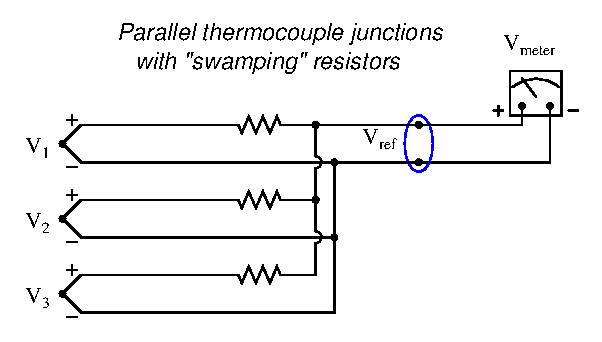
\includegraphics[width=15.5cm]{i00399x02.eps}$$

%(END_ANSWER)





%(BEGIN_NOTES)

Swamping-motstandene ``drukner'' forskjeller i ledermotstand mellom termoelementgrenene. Dette er særlig viktig når kablene har betydelig ulik lengde.

%INDEX% Measurement, temperature: series and parallel thermocouples

%(END_NOTES)
